\par O confinamento quântico é um  dos fenômenos mais estudados em nanotecnologia e é causado pelo confinamento espacial dos portadores de carga em uma ou mais direções por barreiras de potencial (Miller, et al. 1984). O confinamento resulta na mudança de parâmetros referentes à estrutura eletrônica de um material. O tamanho de uma partícula interfere diretamente na sua estrutura de banda e causa mudança nas propriedades do material, como será visto adiante. (Takagahara and Takeda  1992a Wise  2000 Zhao  et  al.  2004).

\par Efeitos quânticos começam a se tornar relevantes quando a dimensão dos pontos quânticos se aproxima do raio de Bohr do éxciton do material na forma bulk (aB). O tamanho do raio de Bohr do éxciton do material bulk pode ser definido\cite{confinamento1} como:

\begin{equation}
	\label{confinamento_1}
	a_{B} = \epsilon \frac{m}{m^{\ast}}a_{0},
\end{equation}
onde $\epsilon$ é a constante dielétrica do material, $m^{\ast}$ é a massa efetiva da partícula, $m$ é a massa do elétron e $a_{0}$ é o raio de Bohr do átomo de hidrogênio.
 
\par O confinamento quântico nos leva a um efeito extremamente relevante para aplicações: o colapso das bandas de energia contínuas para bandas de energia que seguem um padrão discreto e bem definido, semelhante a um átomo, ilustrado na figura X. Para que se entenda o porquê desse efeito de confinamento, vamos analisar o conceito de densidade de estados para os materiais.
%TODO - Conferir referência
\begin{figure}[H]
  \caption{Efeito de confinamento na banda de energia (Adaptado de \cite{bulk2})}
  \centering
  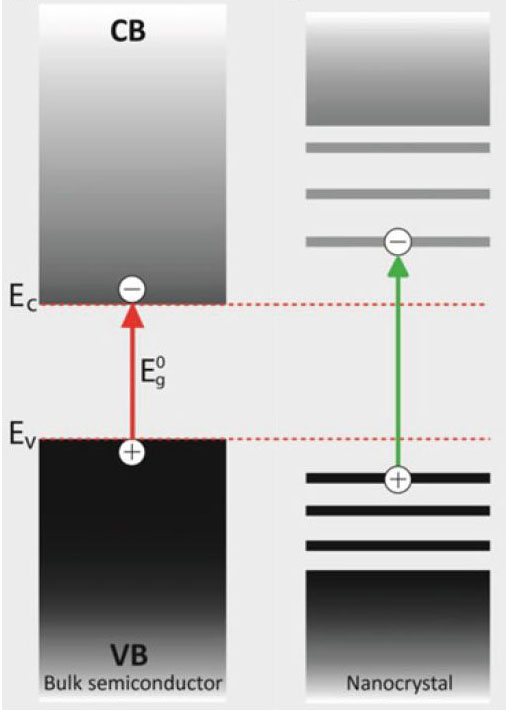
\includegraphics[width=0.5\textwidth]{images/figura9.jpg}
  \label{fig9}
\end{figure}